\documentclass[twocolumn,tighten,dvipsnames,linenumbers]{aastex63}
%\documentclass[modern]{aastex63}
\usepackage{eht,amsmath,gensymb}
\graphicspath{{./}{figures/}}
\usepackage{float}%

% Inline comments
\newcommand\note[1]{{\color{OliveGreen}[note: #1]}}
\newcommand\ckc[1]{{\color{MidnightBlue}[ckc: #1]}}
\newcommand\hyp[1]{{\color{Salmon}[HYP: #1]}}

%==============================================================================
\begin{document}

\title{First Sagittarius A* Event Horizon Telescope Results. V.\\
  Constraining the Astrophysical Properties of the Galactic Center Black Hole}
\author{EHTC et al.}

\shorttitle{First \sgra EHT Results on Astrophysics}
\shortauthors{EHTC et al.}

\submitjournal{ApJL}

\received{\today}
\revised{\today}
%\accepted{\today}

\begin{abstract}
  \color{BrickRed}

  This is a draft for the physical interpretation of EHTC 2017
  campaign data for \sgra.
  Please feel free to add your work and comment on existing notes, but
  DO NOT delete anything without consulting the paper coordinators.

  Tentative title is ``First Sagittarius A* Event Horizon Telescope
  Results. IV. Constraining the Astrophysical Properties of the
  Galactic Center Black Hole''.

  For adding references, simply cite the ADS key, e.g.,
  \texttt{\textbackslash citep\{2019ApJ...875L...5E\}}.
  The bash script \texttt{tools/adsbib.sh} would automatically pull
  the full BibTeX database from ADS.
  See \texttt{Makefile} to learn how to use the scripts in
  \texttt{tools/}.

  \note{The abstract should summarize the scientific outcomes.
    Interesting key questions to address include disk vs jet, or at
    least the range of allowed plasma parameters if \sgra's emission
    comes from the disk vs the parameters if the emission comes from
    the jet(s).
    Note that this may turn into a result on SANE vs MAD and high spin
    vs low spin.}
\end{abstract}

\keywords{black hole, galactic center}

\tableofcontents

%==============================================================================
\section{Introduction
  [Coordinators, Markoff, Ripperda]}
\label{sec:intro}

%------------------------------------------------------------------------------
% Overview

% As a theory paper, we may highlight here that the Galactic Center
% black hole was first predicted theoretically.
The Galactic Center black hole was first predicted theoretically.
By using the black hole model of quasars, \citet{1971MNRAS.152..461L}
predicted that a supermassive black hole (SMBH) would exist at the
center of our Milky Way Galaxy.
Shortly after that, \citet{1974ApJ...194..265B, 1975A&A....43..159E,
  1975ApJ...202L..63L} found the compact radio source now called
Sagittarius~A* (\sgra) at the Galactic Center.
Being our home SMBH, \sgra has continue to be the most studied black
hole candidate since its discovery.

% Theoretical work
On the astrophysics front, \sgra has driven many theoretical
advancements in black hole accretion physics.
For example, the low luminosity of \sgra compared to other quasars
directly inspired the derivation of the Advection-Dominated Accretion
Flow (ADAF) solutions~\citep{1994ApJ...428L..13N, 1995ApJ...444..231N,
  1995ApJ...452..710N, 1996A&AS..120C.287N, 1998ApJ...492..554N}.
Its spectral energy distribution (SED) led to the recognition of
nonthermal electrons' role in hot accretion
flows~\citep{2000ApJ...541..234O}.
Its x-ray observations and early mm-VLBI measurements motivated the
development of the relativistic jet models~\citep{2000A&A...362..113F,
  2004A&A...414..895F, 2005ApJ...635.1203M}.
\note{Please add other theoretical milestones.}
Many of these groundbreak work still define key directions of black
hole research today.

% Numeric work
On the numeric front, after two decades of innovtations, global
general relativistic magnetohdyrodyanmics (GRMHD) simulations
\citep[e.g.,][]{2000ApJ...528..462H, 2003ApJ...589..458D,
  2003ApJ...589..444G, 2007CQGra..24S.235G, 2012ApJS..201....9F,
  2014ApJ...796...22F, 2016ApJS..225...22W, 2017ApJS..231...17A,
  2018JPhCS1031a2008O, 2019A&A...629A..61O, 2019ApJS..243...26P} have
become a standard method to model the dynamic and thermodynamic of
plasma around black holes.
\note{GRMHD code comparison coordinators, please provide proper list
  of references.}
Similarly, there were rapid development in general relativistic ray
tracing (GRRT) \citep[e.g.,][]{1992MNRAS.259..569K,2004MNRAS.349..994B,2007CQGra..24S.259N,2009ApJ...696.1616D,
  2012ApJ...745....1P, 2013ApJ...777...13C,
  2016MNRAS.462..115D, 2016ApJ...820..105P,
  2018MNRAS.475...43M, 2018ApJ...867...59C,
  2018A&A...613A...2B, 2020ApJ...897..148G, 2020arXiv200703045B} and
general relativistic monte carlo radiative transfer
\citep{2009ApJS..184..387D,2013ApJ...777...11S, 2020MNRAS.491.4807M} have enabled us to
convert GRMHD simulations to observables such as SED, images, and
polarization maps.
\note{GRRT code comparison coordinators, please provide proper list of
  references.}
These numerical tools are now used routinely to perform numeric
experiments on \sgra.

% Beyond Einstein and test GR; may leave to the gravity paper
On the gravity front, the facts that radio Very-Long-Baseline
Interferometry~(VLBI) is able to resolve \sgra's predicted black hole
shadow~\citep{2000ApJ...528L..13F} and the shape of the photon ring is
purely a general relativistic effect~\citep{2010ApJ...718..446J} make
\sgra an ideal laboratory to test general relativity in the strong
field regime~\citep{2010ApJ...718..446J, 2014ApJ...784....7B,
  2015ApJ...802...63B, 2015ApJ...814..115P, 2016ApJ...818..121P,
  2016PhRvL.117i1101J, 2019GReGr..51..137P}.
...

%------------------------------------------------------------------------------
% Summarize pervious work

% Modern theoretical + numerical studies
The above developments have led to a large number of studies of
\sgra~\citep[e.g.,][]{2005ApJ...621..785G,2006MNRAS.370..219M, 2007MNRAS.379.1519M,
  2009A&A...508L..13M, 2009ApJ...698..676D, 2009ApJ...701..521C,
  2009ApJ...706..497M, 2012ApJ...746L..10D, 2012MNRAS.421.1315Z,
  2013A&A...559L...3M, 2014A&A...570A...7M, 2014ApJ...790....1B,
  2015A&A...576A..41B, 2015ApJ...799....1C, 2015ApJ...802...69B,
  2015ApJ...812..103C, 2015Sci...350.1242J, 2016A&A...588A..57F,
  2016ApJ...817..173L, 2016ApJ...824...40O, 2016ApJ...826...77B,
  2016ApJ...831....4P, 2016MNRAS.455.2187M, 2017ApJ...837..180G,
  2017ApJ...844...35M, 2017ApJ...851..148M, 2017MNRAS.467.3604R,
  2018A&A...612A..34D, 2018ApJ...856..163M, 2018ApJ...859...60L,
  2018ApJ...863..148P, 2018ApJ...865..104J, 2018ApJ...868..101B,
  2018JCAP...07..015H, 2018MNRAS.478.1875J, 2018MNRAS.478.5209C,
  2019ApJ...881L...2B, 2019ApJ...884..148B, 2019ApJ...886...96H,
  2020ApJ...896L...6R, 2020ApJ...897...99T, 2020MNRAS.492.3272R,
  2020MNRAS.493.1404A, 2020MNRAS.494.4168D, 2020MNRAS.494.5923P,
  2020arXiv200514251B, 2020MNRAS.497.4999D, 2020arXiv200603658P,
  2020ApJ...896L...6R}.
\ckc{Ideally we should cite the above papers in subsequent sections
  and describe why they are relevent to this paper.}
On one hand, due to the richness in accretion and plasma physics, many
of these can only probe a small parameter subspace.
On the other hand, however, even the most sophisticate models to date
are not able to fully explain all the details saw in observations.
\note{Briefly describe main challenges, e.g., constrain electron
  distribution function, model flares.}

%------------------------------------------------------------------------------
% Paper scope

% What EHT brings in
One of the Event Horizon Telescope (EHT) project's main science goals
is to resolve \sgra at horizon scale.
\note{Briefly describe EHT related idea, e.g., resolve the event
  horizon, test general relativity.
  ...}

% Scope of this paper
In this Letter, we scope ourselves on the astrophysics of \sgra.
Given the ambiguity nature of \sgra image using the 2017 EHT
configuration (see Paper II), we combine EHT pre-imaging constraints
and previous observation results to form a robust set of image
independent constraints.
Using analytical and GRMHD models for the accretion flow and GRRT
images calculated from these simulations, we test whether or not the
results of the 2017 EHT observing campaign (hereafter EHT2017) are
consistent with the black hole hypothesis.
Therefore, the results derived from this paper is not affected by
imaging or feature extraction algorithms.
This allows the EHT to cross validate our imaging and feature
extraction results.

% One paragraph summary of the result
\note{One paragraph summary of the result.
  ...}

%------------------------------------------------------------------------------
%\subsection{Notations}

...

Many of them have the common assumption that \sgra is a black hole
described by the Kerr metric, with mass $\mbh$ and dimensionless spin
$\abh$ within the range $-1 < \abh < 1$.
Here $\abh \equiv Jc/G\mbh^2$, where $J$, $G$, and $c$ are the black
hole angular momentum, gravitational constant, and speed of light,
respectively.
We follow the convention of \citetalias{2019ApJ...875L...5E} that
$\abh < 0$ indicate anti-aligned angular momentum between the
accretion flow and that of the black hole.
\note{Describe other details of the current standard \sgra mode, e.g.,
  thick SANE or MAD accretion disks without tilted, etc.
  Describe main controversy in theory/model, e.g., disk vs jet.}

...

%------------------------------------------------------------------------------
%\subsection{Standard Measurement and Assumptions}

We adopted a weighted mean of \citet{2019Sci...365..664D} and
\citet{2019A&A...625L..10G} and fix the mass of \sgra to
\begin{align}
  \mbh &= (4.136 \pm 0.014) \times 10^6 \msun,\\
  D    &= (8.142 \pm 0.023) \kpc.
\end{align}
\note{The \sgra parameter memo indicates that there's no errors in the
  $M/D$ measurements.
  The errors for $M$ and $D$ don't seem consistent.
  Need to check with the parameter definition working group.}

...

%------------------------------------------------------------------------------
%\subsection{One-Zone Model and Estimate}
%\label{sec:onezone}

Using the above mass and distance, the implied characteristic length
is
$G\mbh/c^2 = 6.1 \times 10^{11}\cm$,
characteristic time is
$G\mbh/c^3 = 20.4 \sec$,
angular scale is
$G\mbh/(c^2 D) = 5.03\uas$.
The radius of the shadow is $26.1\uas$.

Then
$ \nu L_\nu
= 4 \pi D^2 \nu F_\nu
= 1.8 \times 10^{34} (D/8127 \pc)^2 \times\allowbreak
  (\nu/230 \GHz)(F_\nu/{\rm Jy}) \erg \sec^{-1}$.
The Eddington luminosity for \sgra is
$ L_\mathrm{Edd}
= 4\pi G\mbh c/\kappa_{es}
= 5.2 \times 10^{44}\allowbreak\erg\sec^{-1}$.
The Eddington accretion rate is
$ \dot\mbh_\mathrm{Edd}
\equiv L_\mathrm{Edd}/(0.1 c^2)
= 5.8 \times 10^{24} \gm \sec^{-1}
= 0.09 \msun \yr^{-1}$.
The Eddington ratio is
$ L_\mathrm{bol}/L_\mathrm{Edd}
= 1.9 \times 10^{-10} (L_\mathrm{bol}/10^{35})$.

Next we consider a one zone model for \sgra.
The model consists of a single temperature sphere with magnetic field
oriented at $\pi/3$ to the line of sight.
Assumed flux is $2\Jy$, which is the average flux for \sgra measured
by ALMA during the 2017 campaign.
The sphere radius is
$5 G\mbh/c^2$.
The ratio of ion to electron temperature
$R \equiv T_i/T_e = 3$.
Assumed plasma
$\beta \equiv P_{gas}/(B^2/(8\pi)) = 1$,
electron temperature
$\Theta_e \equiv k T_e/(m_e c^2) = 10$.

The one zone model flux density is
\begin{align}
  F_\nu = \int I_\nu \, d\Omega =
  \frac{2 k T_e \nu^2}{c^2 D^2} \int dx dy\,\left[1-\exp(-\tau_\nu(x,y)\right]
\end{align}
where $d\Omega$ is a differential solid angle, $x$ and $y$ are
coordinates on the source plane in the same units as $D$, and
$\tau_\nu(x,y) = 2 \alpha_\nu (G\mbh/c^2) \sqrt{X_0^2 - X^2}$,
where $X$ is the offset on the sky from the center of the sphere in
units of
$GM/c^2$, and $X_0 = 5 G\mbh/c^2$.
Finally, $\alpha_\nu$ is the thermal synchrotron absorption
coefficient (units: $\cm^{-1}$).
The density is adjusted until the flux density is $2\Jy$.

For a pure hydrogen model, resulting parameters are: $n_e = 1.1 \times
10^6$, $B = 30\,\mathrm{G}$, $\tau_I = 0.48$, $\tau_Q = 0.35 $,
$\tau_V = 0.27$, Thomson depth $\tau_e = 5 G\mbh/c^2 \sigma_T = 2.2
\times 10^{-6}$, Compton $y = \tau_e 16 \Theta_e^2 = 3.6 \times
10^{-3}$, synchrotron cooling time is $t_{cool} = 3.1 \times 10^4\sec
= 1.5 \times 10^3 G\mbh/c^3$.

There is reason to believe that, if \sgra is fed by stellar winds as
in \citet{2019MNRAS.482L.123R}, the inflowing plasma is almost pure
helium.
In this case the results change only slightly; the cooling time drops
slightly because the rest-mass density (and therefore field strength)
per electron increases.

\note{How good Hung-Yi's one zone model match with Bower et al. 2019?}
\hyp{working on new computation with optical depth analysis as in Bower et al.}

%------------------------------------------------------------------------------
% Organization

This Letter is organized as follows.
\note{...}
In Section~\ref{sec:conclusions}, we summarize our results and discuss
how further analysis of existing EHT data, future EHT data, and
multiwavelength companion observations will sharpen constraints on the
models.
We will also describe a list of open theoretical and numerical
questions that are await of answers.

%==============================================================================
\section{Observational Constraints}
\label{sec:constraints}

In this section, we summarize the observational constraints that will
be used in this paper, which include 320\,GHz VLBI constraints
obtained from the EHT 2017 Observation campaign and previous results.

%------------------------------------------------------------------------------
\subsection{230\,GHz VLBI Pre-Image Size
  [Chan, Chael, Ramakrishnan]}
\label{sec:230size}

\begin{figure*}
  \plotone{sz_grid_gaussian.pdf}
  \caption{...}
  \label{fig:230sz}
\end{figure*}

\begin{figure*}
  \plotone{sz_grid_maxmin.pdf}
  \caption{...}
  \label{fig:230sz}
\end{figure*}

M. Johnson (private communication) reports that the best-fit size of \sgra obtained by measuring the FWHM of a Gaussian fit along a direction 45 deg E of N is approximately $57 \pm 11 \uas$.  This implies $\sigma = 24 \pm 4.7 \uas$.  What is expected from the models?

As a first step, consider the following statistic measured from the image library.  For each image in each model, compute the trace of the second moment tensor, i.e.
\begin{equation}
  R^2 = \frac{1}{F_\nu} \int d\alpha d\beta \, I_\nu \, (\alpha^2 + \beta^2).
\end{equation}
This produces a distribution of characteristic isotropic size $R$ for each model.

We have done a preliminary analysis of $\langle R \rangle$ and $\sigma_R$ for the Illinois segment of the image library, 360 models in all.  The models have  $18.3 \le \langle R \rangle 64.6 \uas$; the smallest is an edge-on SANE, $a = 0.94$ model while the largest is a nearly face-on SANE, $a = -0.94$ model.  Only 22 models have $\langle R \rangle < 30\uas$.  All of these are SANE models, and most have positive spin.  This is in tension with a possible low  asymmetry constraint because this is precisely the set of models with largest asymmetry.

Improvement in analysis: measure the full second moment tensor for each image and produce a distribution of $R$ measured for a random chord drawn across the model.  Since the major and minor axes are likely quite different, at least for some models \citep{2019ApJ...871...30I} this likely relaxes the constraint.  Since the observed size is rather small, this will favor either small models or larger models with a large axis ratio and a particular orientation.

Comment: model size may be sensitive to the presence of a nonthermal tail in the eDF.  The likely sense of the effect is that a nonthermal tail adds millimeter emission at larger radii, making the model larger.  Since most models are already too large, this may constrain the nonthermal tail.

%------------------------------------------------------------------------------
\subsection{230\,GHz VLBI Asymmetry (May not be constraintive)
  [Medeiros, Chan]}
\label{sec:230asym}

Current results from the imaging group suggest \sgra is a surprisingly symmetric ring.   What level of asymmetry is expected in the model library?

To answer this we must first define an asymmetry statistic.  To start, we defined
\begin{equation}
  A = \frac{1}{F_\nu} \int \, d\alpha d\beta \, | I_\nu - {\rm AXI}(I_\nu) |
\end{equation}
where AXI indicates an axisymmetrized version of the image.  We use a crude centering algorithm, and studied only the average image from each model.  This statistic measures how much of the flux is in nonaxisymmetric piece of the image.   The result from measuring $A$ for the average image of the Illinois segment of the \sgra model library is shown in Figure~\ref{fig:asymm}.

\begin{figure*}
  \plotone{asymm.pdf}
  \caption{Asymmetry statistic $A$ for models in the \sgra image library.  Lower $A$ is more symmetric.  All models are more symmetric when viewed nearly face on (or anti-face-on).  The $\Rh = 1$ models exhibit distinct trends and the models will likely be eliminated by other considerations.  For $\Rh \ge 10$ SANE edge-on models are most asymmetric at high positive spin, while the MAD edge-on models are most asymmetric at moderate negative spin.}
  \label{fig:asymm}
\end{figure*}

Improvements in analysis: a better approach to this analysis might be to generate multiple realizations of synthetic data from models, reconstruct an image using one of the imaging pipelines, and measure an asymmetry from the image.  This would produce a distribution $f(A)$ for each model from which a likelihood could be generated.

This should be done for all models in the \sgra image library.

Alternative analysis: one could fit a slashed crescent model to the data and estimate an asymmetry parameter $h$.

%------------------------------------------------------------------------------
\subsection{230\,GHz VLBI Variability
  [Mariyama, Satapathy]}
\label{sec:230variability}

\note{Closure phase variability etc.}

%------------------------------------------------------------------------------
%% \subsection{230\,GHz VLBI Visibility Nulls}
%% \label{sec:230nulls}
%%
%% \note{Identify the possible locations of nulls and use that for a
%%   first pass of model selection.
%%   See, e.g., \citet{2020arXiv200509632P, 2015ApJ...814..115P}.
%%   Look at scatter noise levels etc and identify which part of the
%%   visiblity domain is physically interpretable.}

%------------------------------------------------------------------------------
\subsection{230\,GHz Light Curve Variability
  [Ramakrishnan, Lee, cite TDWG paper]}
\label{sec:230lightcurve}

Because the ALMA light curve is tightly sampled with intervals  between measurements as little as a second and high signal to noise (typically $\sim 60$), it can provide tight new constraints on the high temporal frequency variability of \sgra.  This high frequency variability can also be computed from GRMHD models and compared to the data using various statistics.

An example light curve for 3598 is shown in Figure~\ref{fig:LC3598}.

\begin{figure}
  \plotone{LC_3598.pdf}
  \caption{ALMA lo band light curve for experiment 3598, with Gaussian interpolation and error bars.}
  \label{fig:LC3598}
\end{figure}

V. Ramakrishnan is carrying out an analysis of correlation times and power spectra in the ALMA light curves.

D. Lee and C. Gammie fit the covariance of the ALMA light curve to a Mat\'ern covariance function, which has the form
\begin{equation}
  C(\Delta t) = \mbox{const.} \, \times \, q^\nu K_\nu(q).
\end{equation}
Here $q \equiv \sqrt{2\nu} |\Delta t|/\tau$, $\tau$ is a characteristic timescale, $K_\nu$ is a modified Bessel function, and $\nu$ is a parameter that determines the high frequency falloff of the power spectrum, with $P_\omega \propto \omega^{-2}$ for $\nu = 1/2$.  In general $P_\omega \propto \omega^{-2\nu - 1}$. The special case $\nu = 1/2$ is equivalent to the damped random walk that is commonly used to model AGN light curves, and has been used to model \sgra and \M87's submm light curve. A maximum likelihood fit to the ALMA data yields $\tau \sim 0.9$hr and $\nu \sim 1.5$.

It remains to be seen whether this provides a strong constraint on the models; a preliminary study of model light curves suggests that at least some models are also well fit by a Mat\'ern covariance with similar parameters.

%------------------------------------------------------------------------------
%% \subsection{ALMA Linear Polarization Constraints}
%% \label{sec:polconst}
%%
%% A typical linear polarization fraction for ALMA is $P \sim 6\%$ during the 2017 campaign, with EVPA $\sim -60$deg.  A typical circular polarization fraction is $C \sim 1\%$.  Historical data may also be useful.
%%
%% GRMHD models with fixed eDFs make definite predictions for the distribution of $P$ and $C$.  An example PDF for linear polarization fraction is shown in Figure~\ref{fig:lpexamp}.
%%
%% \begin{figure*}
%%   \plottwo{flin_distr.pdf}{fcirc_distr.pdf}
%%   \caption{Left: distribution of linear polarization fraction from a MAD model with $a = 0$, $i = 30$deg, $\Rh = 10$. Right: distribution of circular polarization fraction for the same model.}
%%   \label{fig:lpexamp}
%% \end{figure*}
%%
%% For the Illinois segment of the \sgra GRMHD models $\< F\>$ varies widely, $\sigma_F/\<F\>$ is typically small or of order $1$, and therefore linear polarization has considerable power to discriminate between models.  The linear polarization fraction varies from $0.08 < \<F\> < 42 \%$.  The smallest $\<F\>$ is in a SANE model with $a = 0$, $i = 90$deg, $\Rh = 10$; $\sigma_F$ for this model is $0.05\%$. The largest $\<F\>$ is in a SANE model with $a = 0.94$, $i = 90$deg, $\Rh = 1$; $\sigma_F$ for this model is $5.2\%$.  All of the highest polarization models have $\Rh = 1$.  Other groups' models should be checked for consistency.
%%
%% The circular polarization in GRMHD models also varies widely, with  $0.09 < \<|C|\> < 3.8 \%$.  The smallest $\<|C|\>$ is in a MAD model with $a = -0.5$, $i = 90$, and $\Rh = 1$.  The largest $\<|C|\>$ is in a SANE model with $a = 0.94$, $i = 50$, and $\Rh = 10$.
%%
%% Comment: this is a very limited set of models.  We may want to consider $R_{low} = 10$ models, as in the \M87 polarization theory effort.   We do not know if the distribution of polarizations is converged, and we do not fully understand sensitivity to all the parameters: this analysis has many of the same issues as the \M87 polarization analysis, except that we know that almost all the flux is compact.

%------------------------------------------------------------------------------
\subsection{86\,GHz Image Size
  [Issaoun, Chan]}
\label{sec:86size}

...

%------------------------------------------------------------------------------
\subsection{Low Frequency SED
  [Chatterjee, Witzel]}
\label{sec:lfconst}

\begin{figure*}
  \plotone{sed.pdf}
  \caption{SED from historical observation and models.}
  \label{fig:SED}
\end{figure*}

\begin{figure*}
  \plotone{sed_grid_zoom.pdf}
  \caption{...}
  \label{fig:SED}
\end{figure*}

Figure~\ref{fig:SED} summarized ...

Purely thermal $\Rh$ eDF models do not match the low frequency SED.

Needed: nonthermal models, or thermal models with an extended isothermal component, that match the SED.

%------------------------------------------------------------------------------
\subsection{NIR (Non-Overproduction) Constraints
  [Modelers and Witzel]}
\label{sec:nirconst}

Although we have relatively little simultaneous NIR data from the 2017 campaign, the NIR lightcurve is observationally well characterized, with NIR flares peaking at $\sim 30$mJy and quiescent flux of order a few mJy.  NIR emission is produced by synchrotron emission in all models that we are aware of.  The NIR/mm color of models is sensitive to the eDF, and in particular nonthermal tails on the eDF, which tend to increase the NIR flux (this point needs to be thoroughly tested).  Thermal eDF models that consistently produce flux densities above a few $mJy$ at K band can therefore be ruled out.

An example analysis based on preliminary NIR images from the Illinois segment of the simulations is presented in Figure~\ref{fig:NIRmodels}.  Evidently $\Rh = 1$ MAD models are strongly disfavored because they overproduce NIR, presumably because they contain more high energy electrons.  A few other models are ruled out, they tend to have large spin and/or be viewed edge on.

\begin{figure*}
  \plottwo{NIR_MAD.pdf}{NIR_SANE.pdf}
  \caption{Left: MAD models, Right: SANE models.  Models marked with a red dot consistently overproduce NIR emission, green dots indicate models that do not overproduce NIR.  The inclination is indicated by the position of the dot, with face-on models near twelve o'clock and edge-on models near three o'clock.}
  \label{fig:NIRmodels}
\end{figure*}

%------------------------------------------------------------------------------
\subsection{X-ray (Non-Overproduction) Constraints
  [Markoff, Witzel, Ripperda, nonthermal group]}
\label{sec:xrayconst}

\begin{figure*}
  \plotone{sed_grid_i70.pdf}
  \caption{SED for different parameters at inclination $i =
    70\degree$.
    The solid black curves take into account all photons---the ones
    originate from synchrotron, bremsstrahlung, and inverse Compton.}
  \label{fig:sed_grid_i70}
\end{figure*}

\begin{figure*}
  \plotone{sed_grid.pdf}
  \caption{SED after applying the x-ray constraints.
    The different colors are for different inclination angles.
    The dotted lines represent the models that fail the x-ray
    constrinat.}
  \label{fig:sed_grid}
\end{figure*}

We are fortunate to have good x-ray coverage on 6 April 2017 from Chandra and NuSTAR.

Rehearse estimates of one-zone emission from thermal synchrotron, Compton scattering, and nonthermal synchrotron.

Model comparison requires computation of SEDs from the models, which are both expensive (they use Monte Carlo to capture Compton scattering) and uncertain (there is evidence that x-ray arises via direct synchrotron from a long tail on the eDF).  C.-K. Chan will compute spectra using {\tt grmonty} and possibly {\tt kmonty} on the OSG.  An example SED is shown in Figure~\ref{fig:SEDexamp}.

%\begin{figure}
%  \plotone{img_Ma+0.94_1900.spectrum_1.0e16_avg.pdf}
%  \caption{Caption}
%  \label{fig:SEDexamp}
%\end{figure}

Nevertheless, it is possible to apply a not-to-exceed threshold constraint similar to that used in the NIR: if a thermal eDF model consistently produces too much x-ray then it can be ruled out.  Early work by \citet{2009ApJ...706..497M} finds that x-ray emission provides a powerful constraint on constant temperature ratio models.

%==============================================================================
\section{Astrophysical Models}

\begin{deluxetable*}{c c c c c}
\tabletypesize{\footnotesize}
\tablehead{
  \colhead{Type} & \colhead{Parameter} & \colhead{Notation} & \colhead{Range/Value(s)} & \colhead{Notes}
}
\startdata
Gravity        & Black Hole Mass                & $M_\mathrm{bh}$      & $4.14\times10^6 M_\odot$            & ... \\
Gravity        & Dimensionless Black Hole Spin  & $a_\mathrm{spin}$    & $-0.94$, $-0.5$, $0$, $0.5$, $0.94$ & ... \\
Fluid          & Magnetization State            & ---                  & MAD, SANE                           & ... \\
Fluid          & Adiabatic Index                & $\Gamma$             & $4/3$, $5/3$                        & ... \\
Fluid          & Evolution time                 & $t$                  & $[5000, 10000] GM/c^3$              & ... \\
Emission Model & Density normalization          & $\rho_\mathrm{unit}$ & Fitted by fixing 230\,GHz flux      & ... \\
Emission Model & Electron-Ion Temperature Ratio & $R_\mathrm{high}$    & 1, 10, 40, 160                      & ... \\
Geometry       & Inclination                    & $i$                  & $10\degree$, $30\degree$, $50\degree$, $70\degree$, $90\degree$ & ... \\
Image          & Image frequency                & $\nu$                & 86\,GHz, 230\,GHz                   & ... \\
Image          & Field of View                  & FoV                  & ...                                 & ... \\
Image          & Pixel size                     & ...                  & ...                                 & ... \\
SED            & SED frequency range            & $\nu$                & ...                                 & ... \\
SED            & SED frequency bin size         & $\Delta\nu$          & ...                                 & ... \\
SED            & SED inclination bin size       & $\Delta\theta$       & ...                                 & ... \\
\enddata
\caption{Parameter space: grid of $5 \times 2 \times 4 \times 5$.}
\label{tab:parameters}
\end{deluxetable*}

...

%------------------------------------------------------------------------------
\subsection{Analytical Accretion Models
  [Pu, Anantua, Jeter]}
\label{sec:anamodels}

\ckc{Should we actually fit ADAF?
  Should we ray trace ADAF?}
\hyp{MCFE is planing to fit ADAF, need to keep update the progress}

...

\cite{Broderick2005} devised a canonical model of Sgr A* as a  radiatively inefficient accretion flow (RIAF). Semi-analytic RIAF models implementing  this using the general relativistic ray tracer GRTRANS \citep{2016MNRAS.462..115D} can be found in  \cite{Emami2021}, where  positrons are included using emission modeling motivated in  \cite{Anantua:2019bna}. The Fig. \ref{fig:EmamiRIAF} model from \cite{Emami2021}  shows Stokes maps and polarized spectra of a \cite{Broderick2005} RIAF with plasma $\beta=10$ and 1$\%$ of the emitting particles nonthermal electrons. The near-extremal ($a/M=0.998$) model shown exhibits Doppler boosting asymmetry in a crescent-shaped intensity pattern with a spiral global electric vector polarization angle (EVPA) pattern and polarization preferentially distributed within this region.


The addition of small non-thermal populations of positrons \citep{Anantua:2019bna,Emami2021} tends to: increase overall intensity in jet regions for fixed electron number density; modify the low-frequency spectral slope; cancel the observed intrinsic circular polarization and enhance circular polarization due to Faraday conversion. The last of these positron effects is particularly apparent when comparing declining tails of x-ray spectra of positron-rich versus positron-poor sources, as seen in Fig. \ref{fig:EmamiRIAFSpectra}.

\begin{figure}%[H]
%   \plotone{RIAFSgrAPlaneTscl1Pt5e11beta1Pt0e01fpos0Pt0fNTH1Pt0e-02copy.png}
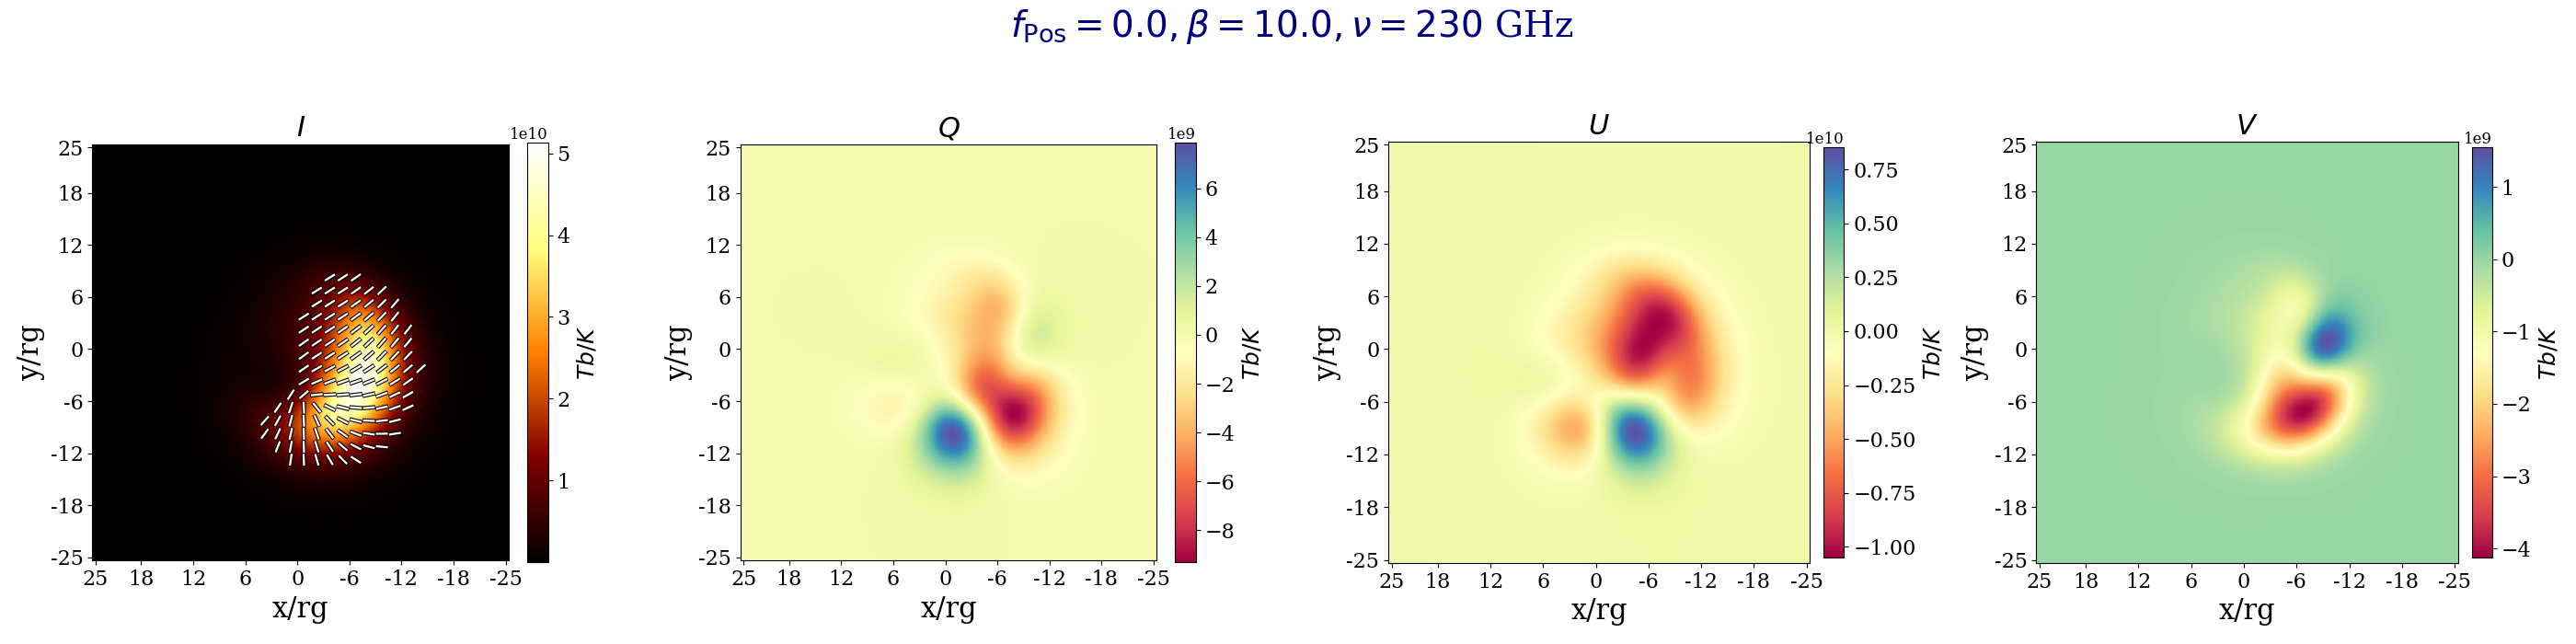
\includegraphics[width=.5\textwidth,height=27mm%,trim=0 380 0 200,clip
]{RIAFSgrAPlaneTscl1Pt5e11beta1Pt0e01fpos0Pt0fNTH1Pt0e-02copy}
  \caption{Polarization maps of Stokes parameters $I$, $Q$, $U$ and $V$ at 230 GHz for a \cite{Broderick2005} RIAF with $\beta=10$.}
  \label{fig:EmamiRIAF}
\end{figure}

\begin{figure}%[H]
%\begin{figure*}%[H]
%   \plotone{RIAFSgrAPlaneTscl1Pt5e11beta1Pt0e01fpos0Pt0fNTH1Pt0e-02copy.png}
  \includegraphics[width=.4\textwidth%width=.55\textwidth,height=25mm%,trim=0 380 0 200,clip
]{PositronModelEtAl2021RIAFPolSpectra%PolSpectscl1Pt5e11Beta1Pt0e1nth1Pt0em2fpos0Pt0
}
  \caption{Polarized SEDs for the Sgr A* RIAF model with  $\beta\in\{10^{-2},10^{0},10^{1}\}$, $f_\mathrm{pos}\in\{0.0,0.5,1.0\}$. The Top Panel shows the Stokes $I$ spectrum, while the Middle Panel shows the SED in linear polarization and the Bottom Panel shows the same for circular polarization.}
  \label{fig:EmamiRIAFSpectra}
%\end{figure*}
\end{figure}

\textcolor{red}{RJA: Include a summary of analytic/semi-analytic models and Sgr A* simulations in the Literature} Analytic disk $\alpha$-model for angular momentum transport \cite{Shakura1973}. Semi-analytic model motivated in \cite{Yuan2003} and expanded in \cite{Broderick2011}. GRMHD Simulation with hotspots reproducing Sgr A* flares \cite{Ripperda2020}.

\note{to be discussed: how much we would like to discuss polarization emission?}\textcolor{red}{RJA: We should mention the M87 Polarization Collaboration papers \cite{EHTCPaperVII}, including a comparison of whether Sgr A* is similar enough (e.g., MAD with vertical fields Faraday depolarized on much of the accretion flow) to have an azimuthally spiral EVPA pattern. Figures in  \citep{Emami2021} have similar morphology}.

\hyp{to-do :  adding historical RIAF fitting result to proto-EHT observations; how recent  GRMHD simulation and subsequent GRRT post-processing suggest other key parameters onto the Broderick 2005 RIAF model; jet componenet? cross referencing MCFE RIAF analysis product?} A proto-EHT array described in \cite{Doeleman2008} estimated the Sgr A* emitting region profile as a circular Gaussian with intrinsic size $37^{+16}_{-10}\ \mu$as.

% EHT flux vs. baseline observations constrain the emitting region intrinsic size to 37 microarcseconds for a circular Gaussian emission profile

More recent measurements of closure phases of a few degrees \cite{Fish2016} suggest an asymmetric ring-like profile, with major axis 56 microarcseconds




%------------------------------------------------------------------------------
\subsection{Numerical Models of the Inner Accretion Flows
  [Mizuno, Wong, Ricarte]}
\label{sec:numodels}

\note{Describe the numerical model and simultion library.}

\ckc{Only study quiescent state for now and leave flare/variability to
  different papers (time domain, MWL, etc)?
  Use slow light only?
  What information should be included for the GRMHD models?
  Boundary conditions, including that at the pole, as which may have
  an effect on the jet.}

%% Propose process:
%% \begin{itemize}
%%   \item Use one zone model to estimate parameters.
%%   \item Use x-ray flux to set bound and rule out part of the
%%     parameter space, especially for amount of non-thermal electrons,
%%     density normalization/accretion rate.
%%     item Use mm--cm flux to constraint electron temperature.
%%   \item ...
%%   \item Use image/ring size to rule score models.
%% \end{itemize}

...

%==============================================================================
%\section{Radiation Models}

%% Abstract thinking: we are trying to connect theory and observation
%% with a vector field $I$, $Q$, $U$, $V$ over 4 dimensions $t$,
%% $\nu$, $\alpha$ (RA), and $\delta$ (dec).
%% For (Fourier) time domain analysis, $t$ is transformed to $\omega$
%% (not to confused with photon frequency $\nu$).
%% For visibility, the $\alpha$ and $\delta$ are transformed into $u$
%% and $v$.
%% These limit what analyses we may do.

%% \ckc{In the origin text, this section should ``summarize main
%%   characteristics that constrain the models.''
%%   But given current structure, it may make sense to reference to the
%%   imaging or MCFE papers for the observational constraints, and just
%%   state these constraints in the next two sections.
%%   We may create a table to summarize these constraints so ``they are
%%   in one place''.}

%% While GRMHD simulations describe the plamas dynamics around black
%% holes, there are more parameters needed to model the black hole images
%% and spectral energy distribution (SED).
%% This is because, obviously, the GRMHD approximaion is scale free in
%% both the black hole mass $\mbh$ and plasma density $\rho_0$.
%% The former allows us to rescale length and time, thereby changing the
%% optical depth; the later allows us to rescale magnetic field strength
%% and energy density, thereby changing the emissivity and absorptivity.

%------------------------------------------------------------------------------
%% \subsection{Phenomenological Models}
%% \label{sec:phenomodels}
%%
%% \ckc{Is this the right place to put disk vs. jet discussion?
%%   How about different favors of hotspot models?
%%
%%   Depending on the development of other papers, it may make sense to
%%   use the fiducial models defined above to guide a reasonable set of
%%   phenomenological models.
%%   And then the actual fits to these phenomenological models may go
%%   into a different, e.g., MCFE, paper.
%%
%%   Recent paper: \citep{2020MNRAS.tmp.2053Y}.}
%%
%% ...

%------------------------------------------------------------------------------
\subsection{Plasma Models
  []}
\label{sec:eDF}

The plasma in the accretion flow around \sgra is mostly collisionless.
This allows electron heating (e.g., accelerated by reconnection) and
cooling (e.g., radiative cooling) mechanism to drive the electrons
away from thermodynamic equilibrium.
Therefore, it is expected that \emph{i}) electrons are cooler than the
ions, and \emph{ii}) the electron distribution function (eDF) is
non-thermal.
The first point was used in \citet{1998ApJ...492..554N} to explain the
spectrum of \sgra.
The second point was used in \citep{2000ApJ...541..234O} to demostrate
that the eDF can signficiant change the predcited properties of \sgra.

Earlier numerical models simply assume a constant ratio between the
electron and ion temperatures \citep{...}.
In order to capture the different physics in the accretion disk and
jets, refined models have been proposed.
This includes using the Bernoulli parameter to distinguish the jet and
the disk \citep{2014A&A...570A...7M}, using the plasma $\beta$
\citep{2015ApJ...799....1C, 2015ApJ...812..103C} with sharp switches, ...

...

\begin{itemize}
\item $\kappa$-model with $\kappa = 5$ everywhere.
\item $\kappa$-model with $\kappa = \kappa(\sigma)$ prescription
  \citep{2016ApJ...826...77B}.
\item Mixed thermal-non-thermal models $\kappa = 3.5$ with $\eta =
  \eta(\sigma)$ using $\Rh$ like prescription; $\eta$ range from 0\%
  to 20\%.
\end{itemize}

...

\begin{figure*}
  \plottwo{Constraints_MAD_nonthermal3.pdf}{Constraints_SANE_nonthermal3.pdf}
  \caption{Left: MAD models, Right: SANE models.  Models marked with a red dot are not satisfying the constraints, while green dots indicate models that are satisfying.  The inclination is indicated by the position of the dot. Each panel is concatenating  the NIR, x-ray (only bremsstrahlung) and 86 GHz(size and flux) constraints. See also Table \ref{tab:nonthermal3}. }
  \label{fig:nonthermal3}
\end{figure*}

%------------------------------------------------------------------------------
\subsection{Ray Traced Images
  []}
\label{sec:images}

...

%------------------------------------------------------------------------------
\subsection{Spectral Energy Distribution
  [Nonthermal group, Moscibrodzka, Cruz-Osorio, Chan]}
\label{sec:SED}

...

%------------------------------------------------------------------------------
%% \subsection{Scattering Models}
%% \label{sec:visibility}

%% ...

%------------------------------------------------------------------------------
%% \subsection{Forward Modeling of Visibility}
%% \label{sec:visibility}

%% ...

%==============================================================================
\section{Comparisons
  [Fromm, Cruz-Osorio, Chatterjee]}
\label{sec:comparisons}

%------------------------------------------------------------------------------
\subsection{Application of Constraints/Image Comparison Metrics/Model Scoring}
\label{sec:apply}

...

%------------------------------------------------------------------------------
%% \subsection{Crescent Fitting}
%% \label{sec:crescent}

%% \note{Use some MCMC framework to fit for crescent models.}

%% ...

%------------------------------------------------------------------------------
%% \subsection{Full Image Comparison}
%% \label{sec:imgconst}

%% \note{Use something like \texttt{nxcorr} or \texttt{nxcinf} to compare
%%   directly the constructed images from the imaging WG and simulations.
%%   Note that the \texttt{nxcorr} family of metrics, as is, do not
%%   capture phases.
%%   Improved metrics are required.
%%   There are also work in developing movie comparison metrics.}

%% ...

%------------------------------------------------------------------------------
%% \subsection{Unsupervised Learning}
%% \label{sec:ml}

%% Apply k-mean clustering (or so) to classify different phenomenological models that satisfy most constraints.

%% Constraints may be multi-messenger, i.e., morphology (asymmetry, compactness, image moments), spectrum (mm, IR, X-Ray), variability, etc. to ensure robustness of the best-bet models selected.

%% Score each category independently and study top sets from each category.  May learn something interesting, e.g., low spin MAD and model X, while show very different images, fit visibility data equally well.

%% ...

%------------------------------------------------------------------------------
%% \Subsection{Perturbative Analysis of Best Fit Models}
%% \label{sec:local-min}

%% Assuming our scoring/fitting methods involve some minimaization of
%% loss/cost/objective function, then the best fits must be local minima
%% (and could be a global minimum).
%% Therefore, it makes sense to perform a pertubative analysis of the
%% local minima and study how the fits change as one varies the weights
%% between the different terms in the loss function.
%% Similar method is proposed by CK in the imaging WG to understand
%% different image reconstructions.

%% ...

%------------------------------------------------------------------------------
\subsection{Pass-Fail Table}
\label{sec:passfail}

...

%------------------------------------------------------------------------------
\subsection{Discussions}
\label{sec:discussions}

...

%------------------------------------------------------------------------------
\subsection{Caveats and Limitations}
\label{sec:caveats}

...

%==============================================================================
\section{Conclusions
  [Coordinators, Markoff, Moscibrodzka]}
\label{sec:conclusions}

...

%------------------------------------------------------------------------------
\subsection{MAD vs SANE}

...

%------------------------------------------------------------------------------
\subsection{Inclination}

...

%------------------------------------------------------------------------------
\subsection{Spin}

...

%==============================================================================
\acknowledgments

Standard EHT acknowledgments.

\vspace{5mm}

\facilities{%
  HST(STIS),
  Swift(XRT and UVOT),
  AAVSO,
  CTIO:1.3m,
  CTIO:1.5m,
  CXO%
}

\software{
  astropy~\citep{2013A&A...558A..33A},
  Cloudy~\citep{2013RMxAA..49..137F},
  SExtractor~\citep{1996A&AS..117..393B}%
}

%==============================================================================
\appendix

\section{Pass/Fail Table}

\begin{deluxetable*}{cccccccccccc}
\tabletypesize{\scriptsize}
\tablehead{
  \colhead{Spacetime} &
  \multicolumn{3}{c}{Fluid} &
  \colhead{Plasma} &
  \multicolumn{6}{c}{Inclinations ($\degree$) that pass constraints} \\
  \colhead{$a_\mathrm{spin}$} & \colhead{Flux} & \colhead{$\Gamma$} & \colhead{Time} & % 3 fluid input
  \colhead{$R_\mathrm{high}$} & % 1 plasma input
  \colhead{86\,GHz}  & \colhead{230\,\mathrm{GHz} 2nd moment} & \colhead{Null Location} & \colhead{$\sigma(230\,\mathrm{GHz})$}  & \colhead{NIR}  & \colhead{X-ray} & \colhead{All} % 4 constraints + 1 combined
}
\startdata
$-0.94$ & MAD  & $5/3$ & ... &   1 & ---         & 70,90       & ---         & ---         & ---         & ---         & \textbf{---        } \\
$-0.94$ & MAD  & $5/3$ & ... &  10 & ---         & 70,90       & 10,30       & ---         & ---         & ---         & \textbf{---        } \\
$-0.94$ & MAD  & $5/3$ & ... &  40 & ---         & 30,50,70,90 & 10,30       & ---         & 10,30       & 10,30,50,70 & \textbf{---        } \\
$-0.94$ & MAD  & $5/3$ & ... & 160 & ---         & All         & 10,30       & ---         & All         & All         & \textbf{---        } \\
$-0.94$ & SANE & $5/3$ & ... &   1 & 70,90       & 70,90       & ---         & ---         & All         & All         & \textbf{---        } \\
$-0.94$ & SANE & $5/3$ & ... &  10 & ---         & 70,90       & ---         & ---         & All         & ---         & \textbf{---        } \\
$-0.94$ & SANE & $5/3$ & ... &  40 & ---         & All         & 30          & ---         & ---         & ---         & \textbf{---        } \\
$-0.94$ & SANE & $5/3$ & ... & 160 & ---         & All         & 10,30       & ---         & All         & All         & \textbf{---        } \\
\hline
$-0.5 $ & MAD  & $5/3$ & ... &   1 & ---         & 50,70,90    & ---         & ---         & ---         & ---         & \textbf{---        } \\
$-0.5 $ & MAD  & $5/3$ & ... &  10 & ---         & 50,70,90    & 10,30,50    & ---         & 10,30,50,70 & All         & \textbf{---        } \\
$-0.5 $ & MAD  & $5/3$ & ... &  40 & 90          & 50,70,90    & 10,30,50    & ---         & All         & All         & \textbf{---        } \\
$-0.5 $ & MAD  & $5/3$ & ... & 160 & All         & All         & 10,30       & ---         & All         & All         & \textbf{---        } \\
$-0.5 $ & SANE & $5/3$ & ... &   1 & 70,90       & 70,90       & ---         & ---         & All         & All         & \textbf{---        } \\
$-0.5 $ & SANE & $5/3$ & ... &  10 & ---         & 50,70,90    & 70          & ---         & All         & ---         & \textbf{---        } \\
$-0.5 $ & SANE & $5/3$ & ... &  40 & ---         & All         & ---         & 10,30,50,70 & All         & ---         & \textbf{---        } \\
$-0.5 $ & SANE & $5/3$ & ... & 160 & ---         & All         & ---         & 10,30,50,70 & All         & All         & \textbf{---        } \\
\hline
$ 0.0 $ & MAD  & $5/3$ & ... &   1 & 70,90       & 30,50,70,90 & ---         & 10,30,50,70 & ---         & ---         & \textbf{---        } \\
$ 0.0 $ & MAD  & $5/3$ & ... &  10 & All         & All         & 10,30       & 10,30,50    & 10,30,50,70 & 10,30,50,70 & \textbf{10,30      } \\
$ 0.0 $ & MAD  & $5/3$ & ... &  40 & All         & 30,50,70,90 & 30          & 10,30,50    & All         & All         & \textbf{30         } \\
$ 0.0 $ & MAD  & $5/3$ & ... & 160 & All         & 30,50,70,90 & ---         & 10,30,50    & All         & All         & \textbf{---        } \\
$ 0.0 $ & SANE & $5/3$ & ... &   1 & 50,70       & 50,70,90    & ---         & ---         & All         & All         & \textbf{---        } \\
$ 0.0 $ & SANE & $5/3$ & ... &  10 & ---         & 30,50,70,90 & 70          & 50,70,90    & All         & ---         & \textbf{---        } \\
$ 0.0 $ & SANE & $5/3$ & ... &  40 & ---         & 30,50,70,90 & ---         & All         & All         & ---         & \textbf{---        } \\
$ 0.0 $ & SANE & $5/3$ & ... & 160 & ---         & 10,30,50,70 & ---         & All         & All         & All         & \textbf{---        } \\
\hline
$ 0.5 $ & MAD  & $5/3$ & ... &   1 & 50,70,90    & All         & ---         & ---         & ---         & ---         & \textbf{---        } \\
$ 0.5 $ & MAD  & $5/3$ & ... &  10 & 30,50,70    & All         & 10,30       & ---         & 10,30       & 10,30,50    & \textbf{---        } \\
$ 0.5 $ & MAD  & $5/3$ & ... &  40 & 30,50,70    & All         & 10,30       & ---         & 10,30,50,70 & All         & \textbf{---        } \\
$ 0.5 $ & MAD  & $5/3$ & ... & 160 & 30,50       & All         & 10,30       & ---         & All         & All         & \textbf{---        } \\
$ 0.5 $ & SANE & $5/3$ & ... &   1 & 50,70       & 50,70,90    & ---         & ---         & All         & All         & \textbf{---        } \\
$ 0.5 $ & SANE & $5/3$ & ... &  10 & ---         & 10,30,50    & ---         & ---         & All         & All         & \textbf{---        } \\
$ 0.5 $ & SANE & $5/3$ & ... &  40 & ---         & All         & 10,30       & ---         & All         & 10,30,50,70 & \textbf{---        } \\
$ 0.5 $ & SANE & $5/3$ & ... & 160 & ---         & All         & 10,30       & ---         & All         & All         & \textbf{---        } \\
\hline
$ 0.94$ & MAD  & $5/3$ & ... &   1 & 70,90       & 30,50,70,90 & ---         & ---         & ---         & ---         & \textbf{---        } \\
$ 0.94$ & MAD  & $5/3$ & ... &  10 & 50,70,90    & All         & 10,30       & ---         & ---         & ---         & \textbf{---        } \\
$ 0.94$ & MAD  & $5/3$ & ... &  40 & 30,50,70,90 & All         & 10,30       & ---         & 10,30       & 10,30,50    & \textbf{---        } \\
$ 0.94$ & MAD  & $5/3$ & ... & 160 & 30,50,70,90 & All         & 10,30       & ---         & All         & All         & \textbf{---        } \\
$ 0.94$ & SANE & $5/3$ & ... &   1 & 10,30,50,70 & 30,50       & ---         & ---         & All         & All         & \textbf{---        } \\
$ 0.94$ & SANE & $5/3$ & ... &  10 & ---         & 10          & 10          & ---         & All         & All         & \textbf{---        } \\
$ 0.94$ & SANE & $5/3$ & ... &  40 & ---         & All         & 10,30       & ---         & All         & All         & \textbf{---        } \\
$ 0.94$ & SANE & $5/3$ & ... & 160 & ---         & All         & 10          & ---         & All         & All         & \textbf{---        } \\
\enddata
\caption{Fixed parameters: black hole mass $M_\mathrm{bh} = 4.14\times10^6 M_\odot$. }
\label{tab:parameters}
\end{deluxetable*}

%Power-law models
%MODEL 1: constant powerlaw index
\begin{deluxetable*}{cccccccccc}
\tabletypesize{\footnotesize}
\tablehead{
  \colhead{Spacetime} &
  \multicolumn{3}{c}{Fluid} &
  \colhead{Plasma} &
  \multicolumn{5}{c}{Inclinations that pass constraints among 10$\degree$, 50$\degree$, 90$\degree$} \\
  \colhead{$a_\mathrm{spin}$} & \colhead{Flux} & \colhead{$\Gamma$} & \colhead{Time} & % 3 fluid input
  \colhead{$R_\mathrm{high}$} & % 1 plasma input
  \colhead{86\,GHz flux}  & \colhead{$\sigma(230\,\mathrm{GHz})$}  & \colhead{NIR flux}  & \colhead{X-ray} & \colhead{All} % 4 constraints + 1 combined
}
\startdata
$-0.94$ & MAD  & $13/9$ & ... &   1 & ---         & ---         & ---         & NA         & \textbf{---        } \\
$-0.94$ & MAD  & $13/9$ & ... &  40 & ---         & ---         & 10          & NA         & \textbf{---        } \\
$-0.94$ & MAD  & $13/9$ & ... & 160 & ---         & ---         & 50          & NA         & \textbf{---        } \\
$-0.94$ & SANE & $5/3$  & ... &   1 & ---         & ---         & 50          & NA         & \textbf{---        } \\
$-0.94$ & SANE & $5/3$  & ... &  40 & 90          & ---         & 10,50,90    & NA         & \textbf{---        } \\
$-0.94$ & SANE & $5/3$  & ... & 160 & 50          & ---         & 50          & NA         & \textbf{---        } \\
\hline
$ 0.0 $ & MAD  & $13/9$ & ... &   1 & ---         & ---         & ---         & NA         & \textbf{---        } \\
$ 0.0 $ & MAD  & $13/9$ & ... &  40 & ---         & ---         & 10,50,90    & NA         & \textbf{---        } \\
$ 0.0 $ & MAD  & $13/9$ & ... & 160 & ---         & ---         & 50          & NA         & \textbf{---        } \\
$ 0.0 $ & SANE & $5/3$  & ... &   1 & ---         & ---         & 50          & NA         & \textbf{---        } \\
$ 0.0 $ & SANE & $5/3$  & ... &  40 & 90          & 10,50,90    & 10,50,90    & NA         & \textbf{90         } \\
$ 0.0 $ & SANE & $5/3$  & ... & 160 & 50          & 50          & 50          & NA         & \textbf{50         } \\
\hline
$ 0.94$ & MAD  & $13/9$ & ... &   1 & ---         & ---         & ---         & NA         & \textbf{---        } \\
$ 0.94$ & MAD  & $13/9$ & ... &  40 & 50,90       & ---         & 10          & NA         & \textbf{---        } \\
$ 0.94$ & MAD  & $13/9$ & ... & 160 & 50          & ---         & 50          & NA         & \textbf{---        } \\
$ 0.94$ & SANE & $5/3$  & ... &   1 & ---         & 50          & 50          & NA         & \textbf{---        } \\
$ 0.94$ & SANE & $5/3$  & ... &  40 & ---         & 10,50,90    & 10          & NA         & \textbf{---        } \\
$ 0.94$ & SANE & $5/3$  & ... & 160 & 50          & ---         & ---         & NA         & \textbf{---        } \\
\enddata
\caption{Non-thermal Power-law model 1: Fixed parameters: black hole mass $M_\mathrm{bh} = 4.14\times10^6 M_\odot$. Note: $\sigma(230\,\mathrm{GHz})$ has been calculated over 5.6 hr.}
\label{tab:parameters}
\end{deluxetable*}

%MODEL 2: variable powerlaw index
\begin{deluxetable*}{cccccccccc}
\tabletypesize{\footnotesize}
\tablehead{
  \colhead{Spacetime} &
  \multicolumn{3}{c}{Fluid} &
  \colhead{Plasma} &
  \multicolumn{5}{c}{Inclinations that pass constraints among 10$\degree$, 50$\degree$, 90$\degree$} \\
  \colhead{$a_\mathrm{spin}$} & \colhead{Flux} & \colhead{$\Gamma$} & \colhead{Time} & % 3 fluid input
  \colhead{$R_\mathrm{high}$} & % 1 plasma input
  \colhead{86\,GHz flux}  & \colhead{$\sigma(230\,\mathrm{GHz})$}  & \colhead{NIR flux}  & \colhead{X-ray} & \colhead{All} % 4 constraints + 1 combined
}
\startdata
$-0.94$ & MAD  & $13/9$ & ... &   1 & ---         & ---         & ---         & NA         & \textbf{---        } \\
$-0.94$ & MAD  & $13/9$ & ... &  40 & 10          & ---         & 10,50       & NA         & \textbf{---        } \\
$-0.94$ & MAD  & $13/9$ & ... & 160 & 50          & ---         & 50          & NA         & \textbf{---        } \\
$-0.94$ & SANE & $5/3$  & ... &   1 & ---         & ---         & 50          & NA         & \textbf{---        } \\
$-0.94$ & SANE & $5/3$  & ... &  40 & ---         & ---         & 10,50,90    & NA         & \textbf{---        } \\
$-0.94$ & SANE & $5/3$  & ... & 160 & ---         & ---         & 50          & NA         & \textbf{---        } \\
\hline
$ 0.0 $ & MAD  & $13/9$ & ... &   1 & ---         & ---         & ---         & NA         & \textbf{---        } \\
$ 0.0 $ & MAD  & $13/9$ & ... &  40 & ---         & ---         & 10,50,90    & NA         & \textbf{---        } \\
$ 0.0 $ & MAD  & $13/9$ & ... & 160 & ---         & ---         & 50          & NA         & \textbf{---        } \\
$ 0.0 $ & SANE & $5/3$  & ... &   1 & ---         & ---         & 50          & NA         & \textbf{---        } \\
$ 0.0 $ & SANE & $5/3$  & ... &  40 & ---         & ---         & 10,50,90    & NA         & \textbf{---        } \\
$ 0.0 $ & SANE & $5/3$  & ... & 160 & ---         & ---         & 50          & NA         & \textbf{---        } \\
\hline
$ 0.94$ & MAD  & $13/9$ & ... &   1 & ---         & ---         & 50          & NA         & \textbf{---        } \\
$ 0.94$ & MAD  & $13/9$ & ... &  40 & 10,50,90    & ---         & 10          & NA         & \textbf{---        } \\
$ 0.94$ & MAD  & $13/9$ & ... & 160 & 50          & ---         & 50          & NA         & \textbf{---        } \\
$ 0.94$ & SANE & $5/3$  & ... &   1 & ---         & ---         & ---         & NA         & \textbf{---        } \\
$ 0.94$ & SANE & $5/3$  & ... &  40 & ---         & 10          & 10          & NA         & \textbf{---        } \\
$ 0.94$ & SANE & $5/3$  & ... & 160 & ---         & ---         & ---         & NA         & \textbf{---        } \\
\enddata
\caption{Non-thermal Power-law model 2: Fixed parameters: black hole mass $M_\mathrm{bh} = 4.14\times10^6 M_\odot$. Note: $\sigma(230\,\mathrm{GHz})$ has been calculated over 5.6 hr.}
\label{tab:parameters}
\end{deluxetable*}


%MODEL 3: Kappa as function of beta and sigma
\begin{deluxetable*}{cccccccccc}
\tabletypesize{\footnotesize}
\tablehead{
  \colhead{Spacetime} &
  \multicolumn{3}{c}{Fluid} &
  \colhead{Plasma} &
  \multicolumn{5}{c}{Inclinations that pass constraints among 10$\degree$, 50$\degree$, 90$\degree$} \\
  \colhead{$a_\mathrm{spin}$} & \colhead{Flux} & \colhead{$\Gamma$} & \colhead{Time} & % 3 fluid input
  \colhead{$R_\mathrm{high}$} & % 1 plasma input
  \colhead{86\,GHz flux and size}  & \colhead{$\sigma(230\,\mathrm{GHz})$}  & \colhead{NIR flux}  & \colhead{X-ray} & \colhead{All} % 4 constraints + 1 combined
}
\startdata
$-0.94$ & MAD  & $4/3$ & ... &   1 & All         & ---         & ---         & 10        & \textbf{---        } \\
$-0.94$ & MAD  & $4/3$ & ... &  40 & All         & ---         & ---         & All       & \textbf{---        } \\
$-0.94$ & MAD  & $4/3$ & ... &  80 & All         & ---         & ---         & All       & \textbf{---        } \\
$-0.94$ & MAD  & $4/3$ & ... & 160 & All         & ---         & All         & All       & \textbf{---        } \\
$-0.94$ & SANE & $4/3$ & ... &   1 & ---         & ---         & All         & All       & \textbf{---        } \\
$-0.94$ & SANE & $4/3$ & ... &  40 & 10,50       & ---         & ---         & All       & \textbf{---        } \\
$-0.94$ & SANE & $4/3$ & ... &  80 & 10          & ---         & ---         & All       & \textbf{---        } \\
$-0.94$ & SANE & $4/3$ & ... & 160 & 10          & ---         & ---         & ---       & \textbf{---        } \\
\hlin
$ 0.0 $ & MAD  & $4/3$ & ... &   1 & All         & ---         & ---         & All       & \textbf{---        } \\
$ 0.0 $ & MAD  & $4/3$ & ... &  40 & All         & ---         & 10,50       & All       & \textbf{---        } \\
$ 0.0 $ & MAD  & $4/3$ & ... &  80 & All         & ---         & All         & All       & \textbf{---        } \\
$ 0.0 $ & MAD  & $4/3$ & ... & 160 & All         & ---         & All         & All       & \textbf{---        } \\
$ 0.0 $ & SANE & $4/3$ & ... &   1 & 10          & ---         & All         & All       & \textbf{---        } \\
$ 0.0 $ & SANE & $4/3$ & ... &  40 & 10,50       & ---         & ---         & All       & \textbf{---        } \\
$ 0.0 $ & SANE & $4/3$ & ... &  80 & 10          & ---         & ---         & All       & \textbf{---        } \\
$ 0.0 $ & SANE & $4/3$ & ... & 160 & 10          & ---         & ---         & ---       & \textbf{---        } \\
\hline
$ 0.94$ & MAD  & $4/3$ & ... &   1 & All         & ---         & ---         & 10,50      & \textbf{---        } \\
$ 0.94$ & MAD  & $4/3$ & ... &  40 & All         & ---         & ---         & All        & \textbf{---        } \\
$ 0.94$ & MAD  & $4/3$ & ... &  80 & All         & ---         & 10          & All        & \textbf{---        } \\
$ 0.94$ & MAD  & $4/3$ & ... & 160 & All         & ---         & 10,50       & All        & \textbf{---        } \\
$ 0.94$ & SANE & $4/3$ & ... &   1 & 10          & ---         & All         & All        & \textbf{---        } \\
$ 0.94$ & SANE & $4/3$ & ... &  40 & 10,50       & ---         & ---         & All        & \textbf{---        } \\
$ 0.94$ & SANE & $4/3$ & ... &  80 & 10          & ---         & ---         & All        & \textbf{---        } \\
$ 0.94$ & SANE & $4/3$ & ... & 160 & 10          & ---         & ---         & ---        & \textbf{---        } \\
\enddata
\caption{Non-thermal Kappa $\kappa=\kappa(\sigma, \beta)$ model 3. All=10,50,90. \textcolor{blue}{Note that the X-ray only consider bremsstrahlung emission.} }
\label{tab:nonthermal3}
\end{deluxetable*}

%==============================================================================
\section{Details ...}
\label{sec:details}

\note{Details that are too long to be included in the main text.}

%------------------------------------------------------------------------------
\subsection{GRMHD Resolution and Convergence}
\label{sec:converge}

\note{Ensure that SANE and MAD simulations are run long enough so the
  accretoin flows reach steady states.
  Cite SANE code comparison paper \citep{2019ApJS..243...26P}, MAD
  code comparison paper (in prep.) and \citet{2012MNRAS.426.3241N,
    2013MNRAS.436.3856S} instead of an appendix?}

%------------------------------------------------------------------------------
\subsection{Image Resolution and Field of View}
\label{sec:res-FoV}

\note{Show work in ``Field-of-View and Resolution Requirements for
  Simulations of Sgr~A*'' Note by Antonios Nathanail, Avery Broderick,
  Charles Gammie, Dimitrios Psaltis, Dom Pesce, George Wong, Lindy
  Blackburn, Michael Johnson, Yosuke Mizuno, Zachary Gelles, et al;
  cite \citet{2020arXiv200406210P}.}

%------------------------------------------------------------------------------
\subsection{Samping SED}
\label{sec:sed-sample}

\begin{figure*}
  \plotone{lightcurves.pdf}
  \caption{X-ray lightcurves.}
  \label{fig:lc}
\end{figure*}

\begin{figure}
  \plotone{sed_Ma0_hist.pdf}
  \caption{X-ray histogram.}
  \label{fig:hist}
\end{figure}

%------------------------------------------------------------------------------
%% \subsection{Fast Light vs Light-Speed Light}
%% \label{sec:lightspeed}
%%
%% \note{Show Boris Georgiev et al.'s result on comparing fast vs slow
%%   light in GRRT; justify that fast light is a fine approximation for
%%   this work.}

%==============================================================================
%% \section{Correspondence Principle in Scoring}
%% \label{sec:correspondence}
%%
%% \note{Answer the questions ``if a model fits the data with a simple
%%   metric, what's the implication to a more complicated metric?''
%%   and ``if a model fits the data with a complicated metric, does it
%%   always score well in a simple metric?''}

%==============================================================================
\bibliographystyle{aasjournal}
\bibliography{main}

%==============================================================================
\end{document}
